\begin{figure} [H]
	\centering
	\begin{subfigure}{.49\textwidth}
		\centering
		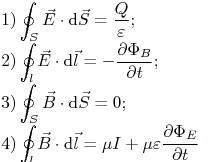
\includegraphics[width=1.0\linewidth]{generalIssues/Figures/maxwell1.png}
		\caption{Postać całkowa.}
		\label{n1}
	\end{subfigure}
	\begin{subfigure}{.49\textwidth}
		\centering
		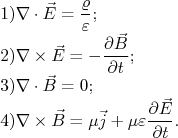
\includegraphics[width=1.0\linewidth]{generalIssues/Figures/maxwell2.png}
		\caption{Postać różniczkowa.}
		\label{r1}
	\end{subfigure}
	\caption{Równania Maxwella.}
	\label{maxwell}
\end{figure}

Rysunek~\ref{maxwell} przedstawia równania Maxwella, gdzie:\newline
$ \varrho $ - gęstość ładunku,\newline
$ \varepsilon $ - przenikalność dielektryczna,\newline
$ \mu $ - przenikalność magnetyczna,\newline
$ \vec{j} $ - gęstość prądu,\newline
$ \Phi_B $- strumień indukcji magnetycznej,\newline
$ \Phi_E $- strumień natężenia pola elektrycznego,\newline
$ \nabla * \vec{F} = \frac{\partial F_x(x,y,z)}{\partial x} + \frac{\partial F_y(x,y,z)}{\partial y} + \frac{\partial F_z(x,y,z)}{\partial z}$ - dywergencja pola wektorowego $ \vec{F} = [F_x, F_y, F_z] $,\newline
$
\nabla \times \vec{F} = 
\begin{vmatrix}
\textbf{i} & \textbf{j} & \textbf{k} \\ 
\frac{\partial}{\partial x} & \frac{\partial}{\partial y} & \frac{\partial}{\partial z} \\ 
F_x & F_y & F_z  \notag
\end{vmatrix}
= (\frac{\partial F_z}{\partial y} - \frac{\partial F_y}{\partial z})\textbf{i} + (\frac{\partial F_x}{\partial z} - \frac{\partial F_z}{\partial x})\textbf{j} + (\frac{\partial F_y}{\partial x} - \frac{\partial F_x}{\partial y})\textbf{k}
$ - rotacja pola wektorowego $ \vec{F} $.\newline

Sens fizyczny praw Maxwella:
\begin{enumerate}[1)]
	\item \underline{Prawo Gaussa dla elektryczności} - źródłem pola elektrycznego są ładunki, a strumień tego pola przez dowolną powierzchnię zamkniętą zależy tylko od ładunku zamkniętego przez tę powierzchnię.
	\item \underline{Prawo Faradaya} - zmiana strumienia indukcji magnetycznej przez powierzchnię zamkniętej pętli powoduje powstanie w tej pętli siły elektromotorycznej indukcji (SEM), a kierunek płynącego prądu jest taki, żeby przeciwdziałać zmianom powodującym indukcję (reguła Lenza).
	\item \underline{Prawo Gaussa dla magnetyzmu} - nie istnieją ładunki magnetyczne, a strumień pola magnetycznego przez dowolną powierzchnię zamkniętą jest równy 0.
	\item \underline{Prawo Ampere'a} - zmienne pole elektryczne i płynący prąd powodują powstanie pola magnetycznego.
\end{enumerate}

Dla fali elektromagnetycznej w próżni wektory $ \vec{E} $ i $ \vec{B} $ drgają w płaszczyznach wzajemnie prostopadłych i dla fali rozchodzącej się w kierunku osi x możemy przyjąć taki układ odniesienia aby wektor $ \vec{E} $ drgał w kierunku osi y a wektor $ \vec{B} $ w kierunku osi z. Zatem wektory $ \vec{E} $ i $ \vec{B} $ mają tylko po jednej składowej:\newline
$ \vec{E} = [0, E, 0] $,\newline
$ \vec{B} = [0, 0, B] $.\newline
Liczmy rotację wektorów $ \vec{E} $ i $ \vec{B} $ (wykorzystując fakt, że nasza fala jest falą płaską i pola $ \vec{E} $ i $ \vec{B} $ zmieniają się tylko względem współrzędnej x, czyli że $ \frac{\partial E}{\partial z} = 0, \frac{\partial B}{\partial y} = 0$):\newline
$ \nabla \times \vec{E} = \textbf{k}\frac{\partial E}{\partial x} $,\newline
$ \nabla \times \vec{B} = -\textbf{j}\frac{\partial B}{\partial x} $.\newline

Korzystając z równań Faradaya oraz Ampera w postaci różniczkowej otrzymujemy (poszukujemy równania dla fal elektromagnetycznych rozchodzących się w próżni gdzie nie będą występowały prądy przewodzenia, czyli $ \vec{j} $ = 0):\newline
$ \textbf{k}\frac{\partial E}{\partial x} = -\frac{\partial \vec{B}}{\partial t} = -\textbf{k}\frac{\partial B}{\partial t} $,\newline
$ \textbf{j}\frac{\partial B}{\partial x} = -\mu_0 \epsilon_0 \frac{\partial \vec{E}}{\partial t} = -\textbf{j} \mu_0 \epsilon_0 \frac{\partial E}{\partial t} $.\newline
W efekcie dostajemy układ dwóch równań:\newline
$ \frac{\partial E}{\partial x} = -\frac{\partial B}{\partial t} $,\newline
$ \frac{\partial B}{\partial x} = - \mu_0 \epsilon_0 \frac{\partial E}{\partial t} $.\newline

Równania falowe dla $ \vec{E} $ i $ \vec{B} $ będą miały identyczną postać. Jeżeli zdecydujemy się szukać równania dla $ \vec{E} $, to eliminujemy z naszego układu równań $ \vec{B} $ przez utworzenie pochodnych mieszanych $ \vec{E} $ względem x i t. Różniczkujemy zatem pierwsze równanie po x, a drugie po t (jeśli chcemy szukać równania dla $ \vec{B} $ eliminujemy w ten sam sposób z naszych równań $ \vec{E} $):\newline
$ \frac{\partial^2 E}{\partial x^2} = -\frac{\partial^2 B}{\partial t \partial x} $,\newline
$ \frac{\partial^2 B}{\partial t \partial x} = - \mu_0 \epsilon_0 \frac{\partial^2 E}{\partial t^2} $.\newline
Z powyższego układu równań otrzymujemy poszukiwane równanie falowe dla pola $ \vec{E} $:\newline
$ \frac{\partial^2 E}{\partial x^2} - \mu_0 \epsilon_0 \frac{\partial^2 E}{\partial t^2} = 0 $\newline
Znając ogólną postać równania falowego dla fali rozchodzącej się z predkością v w kierunku osi x:\newline
$ \frac{\partial^2 \xi}{\partial x^2} - \frac{1}{v^2} \frac{\partial^2 \xi}{\partial t^2} = 0 $\newline
otrzymujemy związek pomiędzy prędkością światła w próżni (c) a wartościami przenikalności elektrycznej i magnetycznej próżni: \newline
$ c = \frac{1}{\sqrt{\mu_0 \epsilon_0}} $.\newline
Rozwiązanie równania falowego dla pola $ \vec{E} $ ma postać:\newline
$ \vec{E} = \vec{E_0}\sin(kx - \omega t) $,\newline
gdzie: $ k = \frac{2\pi}{\lambda} $, $ \omega = ck $.